\documentclass{article}
\usepackage{../fasy-hw}
\usepackage{ wasysym }

%% UPDATE these variables:
\renewcommand{\hwnum}{n+1=8}
\title{Advanced Algorithms, Homework \hwnum}
\author{TODO-Put Your Name Here}
\collab{n/a}
\date{due: 23 November 2020}

\begin{document}

\maketitle

This homework assignment should be
submitted as a single PDF file to to Gradescope.

Write a two-page paper describing to me how you have grown as a student,
computer scientist, mathematician, engineer, or a researcher in this class, and
more generally, in this semester.  To support your argument, you should include
your homework or writing samples (or excerpts from them) in an appendix as
evidence (and reference them!)

If you do not feel that you've grown, explain why.

Remember, style counts. Use complete sentences.

This HW will be graded on the following scale:
\begin{itemize}
    \item No submission (-1 point)
    \item Low pass (+1 point)
    \item Pass (+3 points)
    \item High Pass (+5 points)
\end{itemize}
\newpage

Gosh I know the intention of this one was to get us thinking, but I really got thinking.
\section*{Commentary}
It could be argued the driving force of the university system at large is
a common desire for personal growth. The hope would obviously be to, even if accompanied by catastrophe, develop some aspect of yourself during each course. One thing I very recently noticed is every course I have taken from Brittany seems tailored to probe and challenge each student's goals. 
The first assignment at the beginning of the semester tried to get us to define what our goals for the course were - be it skills or a check mark on degreeworks(figure 1). One metric for gauging this growth, I suppose, would be to see if my answers to these preliminary questions change at all - and I do think they would. The interesting part of growth, though, is it is totally state dependent. Obviously(?) the person I was at the start of the semester is some sort of subset of who I am now, but that does not mean my goals then were inalid or wrong. Anyways, lets dive into the list of things I think I developed as a person!

\section{Algorithms}
The staple development. I was briefly exposed to algorithm proofs from Computational Topology, but I definitely wanted a more thorough exploration of standard techniques involved in verifying algorithms. The big ideas I learned are encompassed in the techniques used to prove correctness and termination of a wide variety of algorithms. I know I mentioned it in previous assignments, but I do like loop invariants a lot. When writing code it is so easy to start slinging out code without thinking too much about why it is right, at least for me. I can always convice myself it is correct, but pinning down the justification in a communicable way is really cool to me. Other examples include the exchange principle and stochastic expected runtime algorithms. 

\section{Communication}
Can anybody really overstate the importance of communication. David A. once toldour class he thought the most impactful invention ever concieved by mankind was the alphabet (or language). I do think it is a kind of intimidating thought experiment to imagine life in a time where the forefront of research was developing a standard of noises that determine the conduit of thought and all meaning. In this course, though, I think it is clear I have been able to improve my communication. One of my biggest weaknesses (ONLY weaknesses ;) ) has always been my ability to get people up to speed with where my mental train of thought is headed. I think my exposure to abstract math and algorithms has probably helped most in reigning in this weakness, but there were several classes where I really think I improved my proofs and reasoning. Evidence in this success is my scores on my proofs. Traditionally, I would get at least one or two junk proofs in a semester but this time around I got none!!! My impressive homework grades are a result of another of my trademark characteristics $\#-5/5$ $\#didn'tdothepiazzaposts$ $\#missedhomework6$ $\#sleep>>notsleep$. 
Finally I have to note the conversation we had about how to be sure a proof is complete. The idea here was I noticed I often times find one property of a problem and run away with it. I make some conclusions based on the assumption where the property I found completely describes the problem. This is obviously not always true, however, and I think the discussion we had about restricting degrees of freedom is a good analysis tool to have in my back pocket. 




\section{Writing} 
Every class includes writing of some sort and when I am writing for you, I do not forget my lessons... You may be wondering what I am talking about here... But let me ask you this question - How many times have you seen me start a sentence with 'This' or 'There' throughout the semester??? BOOM. The clarity has been permanently improved. Not really a direct consequence of the course, but in a sense it kind of is. 

\section{Student}
I need no introduction to make the claim I have historically been a less than ideal student. By this I mean slacking off on both attendance and homeworks. The only way I was able to stay afloat in school was because I got lucky. The cool thing right now, though, is I think my poor student days may be over. Just in time too, because I get to graduate soon (sarcasm)! I really can't say it was anything in particular relation to this course, but it is kind of a big deal for my future. My diagnosis was poor organization/time management which can obviously be seen based on the stunning lack of piazza posts on my homework. However, you can clearly see towards the end of the semester where my attendance stopped flaking. Honestly I think this was the main thing holding me back as a person so I am kind of psyched haha. 

\section{Suggestions}
I know one of the major things I wanted to learn about but didnt get a chance to was algorithm approximation. Talking about theoretical optimums and perturbation theory would be a super awesome course in my opinion, and I think it definitely has the potential to fall under the jurisdiction of 432. 

Hopefully I have successfully hit 2 pages here. Thanks for the great course, as per usual, and have a FAN-TASTIC break/snowmester, whichever boat you managed to land on. 



\section{index}

\begin{figure}

	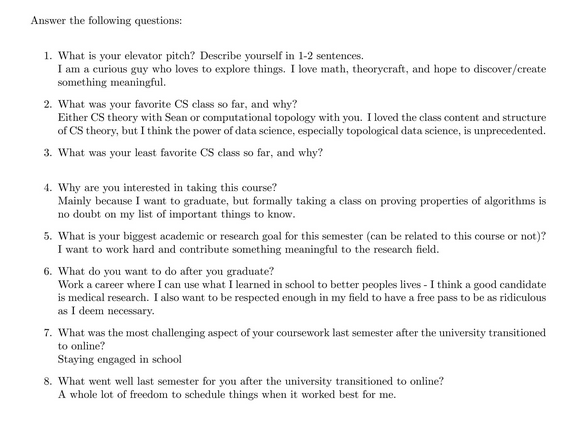
\includegraphics[width=\textwidth]{algos1.png}
	\caption{Homework1 goals}

\end{figure}

\begin{figure}

	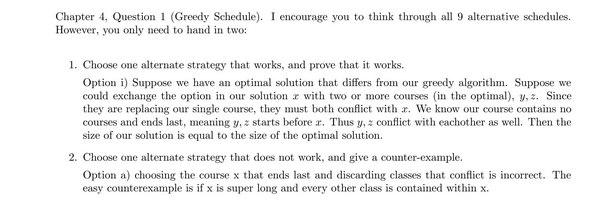
\includegraphics[width=\textwidth]{algos2.png}
	\caption{Homework 5 Example proof}

\end{figure}

\begin{figure}

	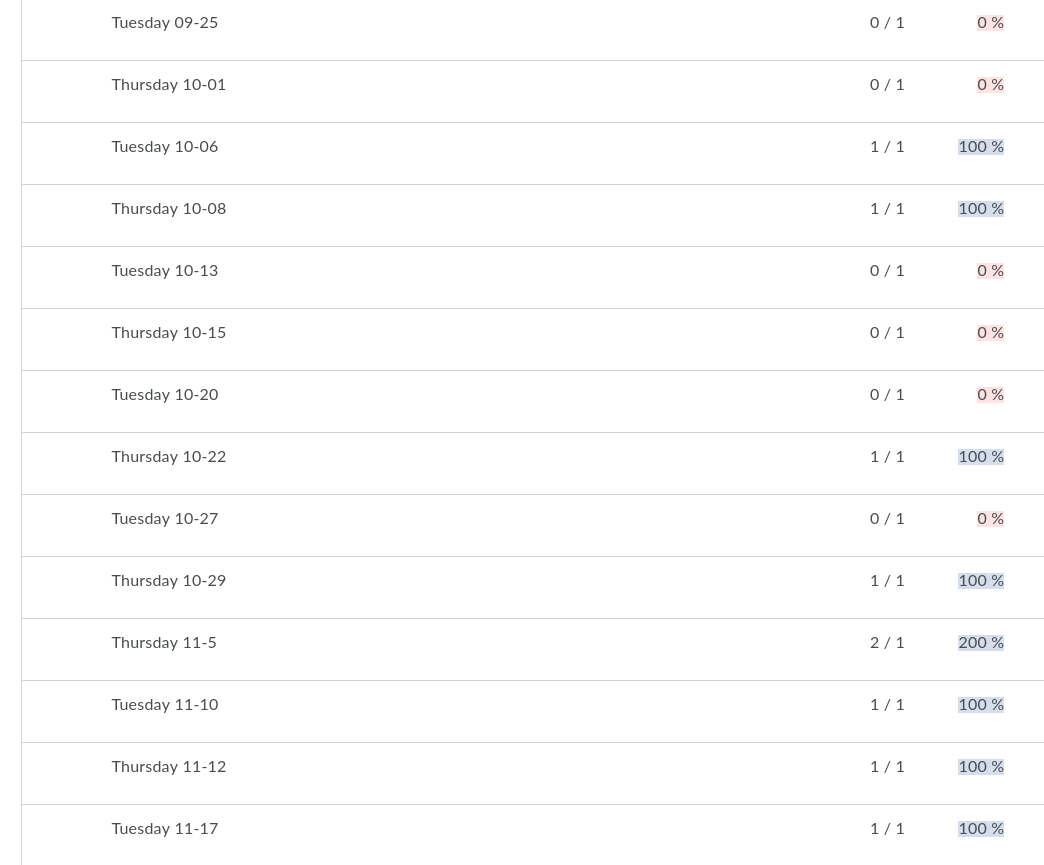
\includegraphics[width=\textwidth]{algos3.png}
	\caption{My attendance towards the end of the semester}


\end{figure}


\end{document}
